\documentclass[12pt]{article}



\linespread{1.25}
\usepackage{float}
\usepackage{hyperref}
\usepackage{graphicx}
\usepackage[notes,backend=biber]{biblatex-chicago}
\usepackage[a4paper,top=3cm,bottom=2.5cm,left=3cm,right=4cm,marginparwidth=1.75cm]{geometry}
\usepackage{tgtermes} % times font
\bibliography{main}
\begin{document}

\section{Alkoholkonsum in Baden Württemberg}



\subsection{Im zeitlichen Verlauf}
Schon im alten Griechenland wird in vielen Erzählungen über Saufgelage berichtet (TODO Quelle), damals war der Alkohol im Alltag allerdings verpönt (TODO Quelle). Erst seit dem Mittelarlter spielt Alkohol eine große Rolle in Europa. Ab dem ?? Jahrhundert wird er als ein wichtiger Teil der Ernährung von allen Altersgruppen mit etwa 3 Litern täglich Konsumiert (TODO Quelle). Man muss aber beachten, dass die Art dies Alkohols, die damals konsumiert wurde stark von heute abweicht. Ein großer Teil des Alkohols wurde z.B. in Form von Biersuppen konsumiert (TODO Quelle), bei deren Kochvorgang allerdings der Alkoholgehalt stark sank (TODO Quelle). Zu Beginn des 17. Jahrhunderts verbreiteten sich neue Genussmittel wie Kaffee, Kakao und Zucker in Europa, was zu einem starken Abfall des Alkoholkonsums führte (TODO Quelle). 

\subsection{Im Vergleich zu anderen Bundesländern}
Viele haben das Vorurteil, dass zwischen dem Trinkverhalten in den nördlichen und den südlichen Bundesländern in Deutschland ein großes Gefälle besteht. Ein Beispiel dafür ist zum Beispiel das bayrische Oktoberfest, bei dem enorme Mengen an Alkohol konsumiert werden. Es wird auch als das größte Drogenfestival in Deutschland bezeichnet (TODO Quelle). Die Wissenschaft ist sich allerdings uneinig ob dieses Vorurteil wirdklich zutrifft. Es gibt Studien die behaupten, dass es durchaus ein Gefälle zwischen dem Trinkverhalten im Norden und im Süden Deutschlands gibt \autocite{meyer_regionale_1998}. Eine andere Studie behauptet wiederum, dass diese Differenzen nur durch falsche Datenerhebung hervorgerufen werden \autocite{kraus_einfluss_2001}. Um diese Behauptungen genauer zu analysieren haben wir die Methoden dieser Studien untersucht: 
\subsubsection {}
Dafür müssen wir zuerst definieren, welche Bundesländer zu Nord- und Süd- Deutschland gehörren.... 
Metrik mit der gemessen wird: Menge an konsumiertem Reinalkohol (pro Trinktag ??)
....
Ergebnis: Es gibt keine Messbare differenz in der Menge an konsumierten reinalkohol zwischen Nord und Süddeutschland
---

Wenn man allerdings die einzelnen Bundesländer genauer betrachtet fällt auf, dass in Bayern tatsächlich überdurchschnittlich viel Alkohol konsumiert wird \autocite{kraus_einfluss_2001}. In Baden Württemberg wird allerdings durchschnittlich relativ wenig Alkohol pro Tag getrunken. Auch der riskante Alkoholkonsum ist relativ gering. Da wir uns in unserer Seminararbeit hautpsächlich auf den Alkoholkonsum von Jugendlichen fokussieren wollen wäre eine Statistik zum durchschnittlichen Alkoholkonsum von Jugendlichen in den verschiedenen Bundesländern natürlich interessant. Bei unserer Rechere haben wir eine solche spezifische Statistik allerdings nicht gefunden. 

Um aber trotzdem eine Aussage über den Alkoholkonsum von Jugendlichen in Deutschland zu treffen, haben wir die Daten auf der Plattform GENESIS (Gemeinsames Neues Statistisches Informations-System) \autocite{noauthor_statistisches_nodate} verwendet. Auf GENESIS findet sich ein breit  gefächertes Datenangebot von den statistischen Landesämtern und dem Statistischen Bundesamt. Dieses enthält u.a. einen Datensatz mit dem Bundesland, Alter, Geschlecht und der Hauptdiagnose aller Krankenhauspatienten in Deutschland \autocite{noauthor_genesis_nodate}. Aus dieser Statistik haben wir alle Krankenhausaufenthalte von Jugendlichen bis 19 Jahren, die aufgrund von einer Alkoholintoxikation (Diagnose ICD-10 F10.0 \autocite{noauthor_icd-10-code_nodate}) im Krankenhaus waren extrahiert. In der folgenden Grafik sieht man diese im Durchschnitt pro 100.000 Einwohner des jeweiligen Bundeslandes über die letzten 15 Jahre aufgelistet.

\begin{figure}[H]
    \centering
    \includegraphics[scale=.7]{"assets/Alkohol_Bundesländer_avg_15_Jahre.png"}
    \caption{Alkoholbedingte Krankenhausaufenthalte von Jugendlichen in Abhängigkeit des Bundeslandes}
    \label{fig:Krankenhausaufenthalte_1}
\end{figure}

Für die Bevölkerungsanzahlen zur normalisierung der Statistik wurde die Bevölkerung des jeweiligen Bundeslandes zum jeweiligen Zeitpunkt verwendet \autocite{noauthor_statistisches_2024}. Die Werte wurden mit Python berechnet und die Grafik wurde mit der Python Bibliothek Matplotlib \autocite{noauthor_matplotlib_nodate} erstellt. 

Es fällt auf, dass die Werte für kleine Bundesländer (Saarland, Hamburg und Berlin) stark abweichen. Das könnte an den geringen Fallzahlen liegen, die dann zu Extremwerten führen. Die absoluten Fallzahlen schwanken im zum Beispiel Saarland über die Jahre von 200 bis knapp 400. Ein weiterer wichtiger Aspekt, der bei der Analyse dieser Daten beachtet werden muss, ist der Länderaustausch von Patienten. Das Bundesland, in dem ein Patient behandelt werden muss, muss nicht mit dem Wohnort des Patienten übereinstimmen. Das kann aufgrund der normalisierung der Daten zu einer verfälschung der Ergebnisse führen. Auf GENESIS ist auch eine Statistik verfügbar, die statt dem Ort des Krankenhauses den Wohnort der Patienten angibt \autocite{noauthor_genesis_nodate-1}.

\begin{figure}[H]
    \centering
    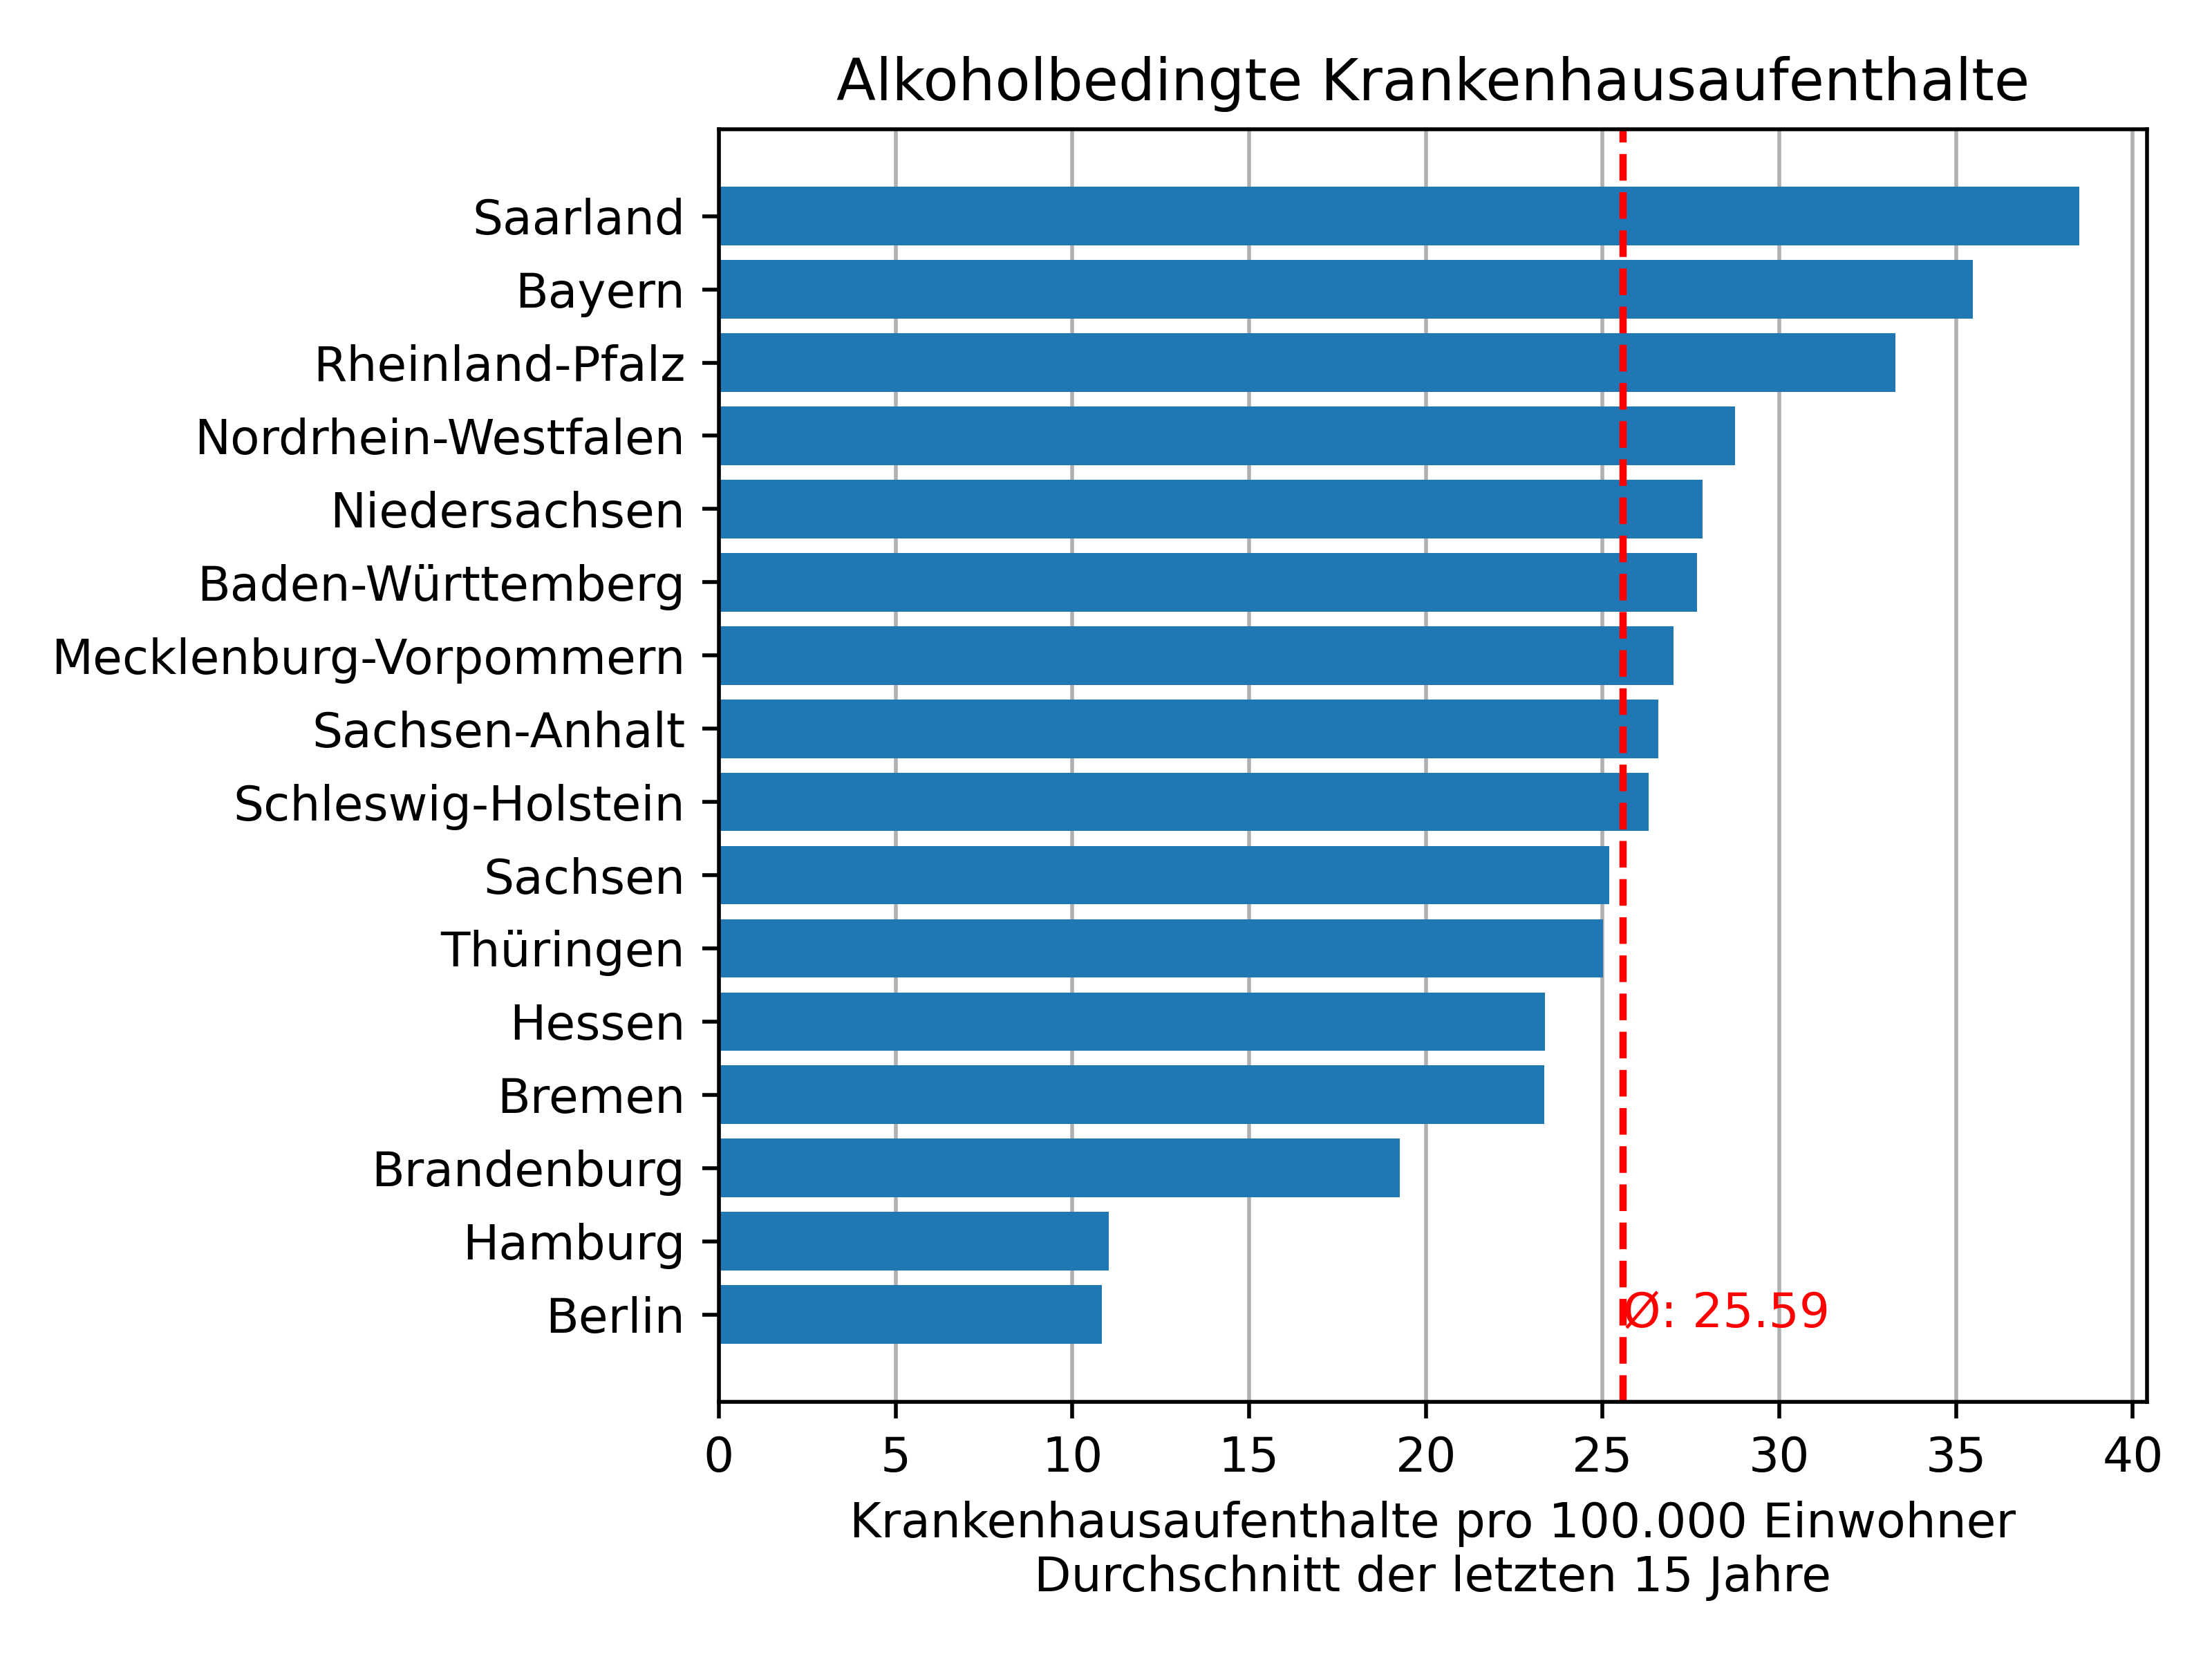
\includegraphics[scale=.7]{"assets/Alkohol_Wohnort_avg_15_Jahre.png"}
    \caption{Alkoholbedingte Krankenhausaufenthalte von Jugendlichen in Abhängigkeit des Wohnortes}
    \label{fig:Krankenhausaufenthalte_2}
\end{figure}

Grafik \ref{fig:Krankenhausaufenthalte_2} wurde mit den gleichen Methoden wie Grafik \ref{fig:Krankenhausaufenthalte_1} erstellt. Patienten deren Wohnort unbekannt ist und Patienten, die aus dem Ausland kommen wurden ignoriert. 
Die Werte für die meisten größeren Bundesländer sind nahezu gleich geblieben, da dort der Anteil der Patienten, die in einem anderen Bundesland behandelt wurden im vergleich zu den Patienten, die in ihrem Heimatbundesland behandelt wurden sehr klein ist. Die Werte der kleineren Bundesländer (Hamburg, Berlin, Bremen und Saarland) sind dagegen stärker gesunken, vor allem bei Bremen. Das könnte daran liegen, dass ein Teil der Patienten, die zum Beispiel in einem Krankenhaus in Bremen behandelt wurden aus dem umliegenden Niedersachsen kommen. Dass die hohen Werte im Saarland kein Fehler in der Statistik sind, sondern ein reales Problem darstellen zeigt sich auch in diesem Artikel \autocite{noauthor_saarland_nodate}, der das Problem des alkoholmissbrauchs von Jugendlichen im Saarland beschreibt. 
\\\\\\
Grafik \ref{fig:Krankenhausaufenthalte_1} und Grafik \ref{fig:Krankenhausaufenthalte_2} stellen den Durchschnitt der alkoholbedingten Krankenhausaufenthalte über die letzten 15 Jahre dar. Die folgende Grafik beschäftigt sich dagegen mit dem Zeitlichen Verlauf der alkoholbedingten Krankenhausaufenthalte in Baden-Württemberg und in Deutschland von 2000 bis 2022.
\begin{figure}[H]
    \centering
    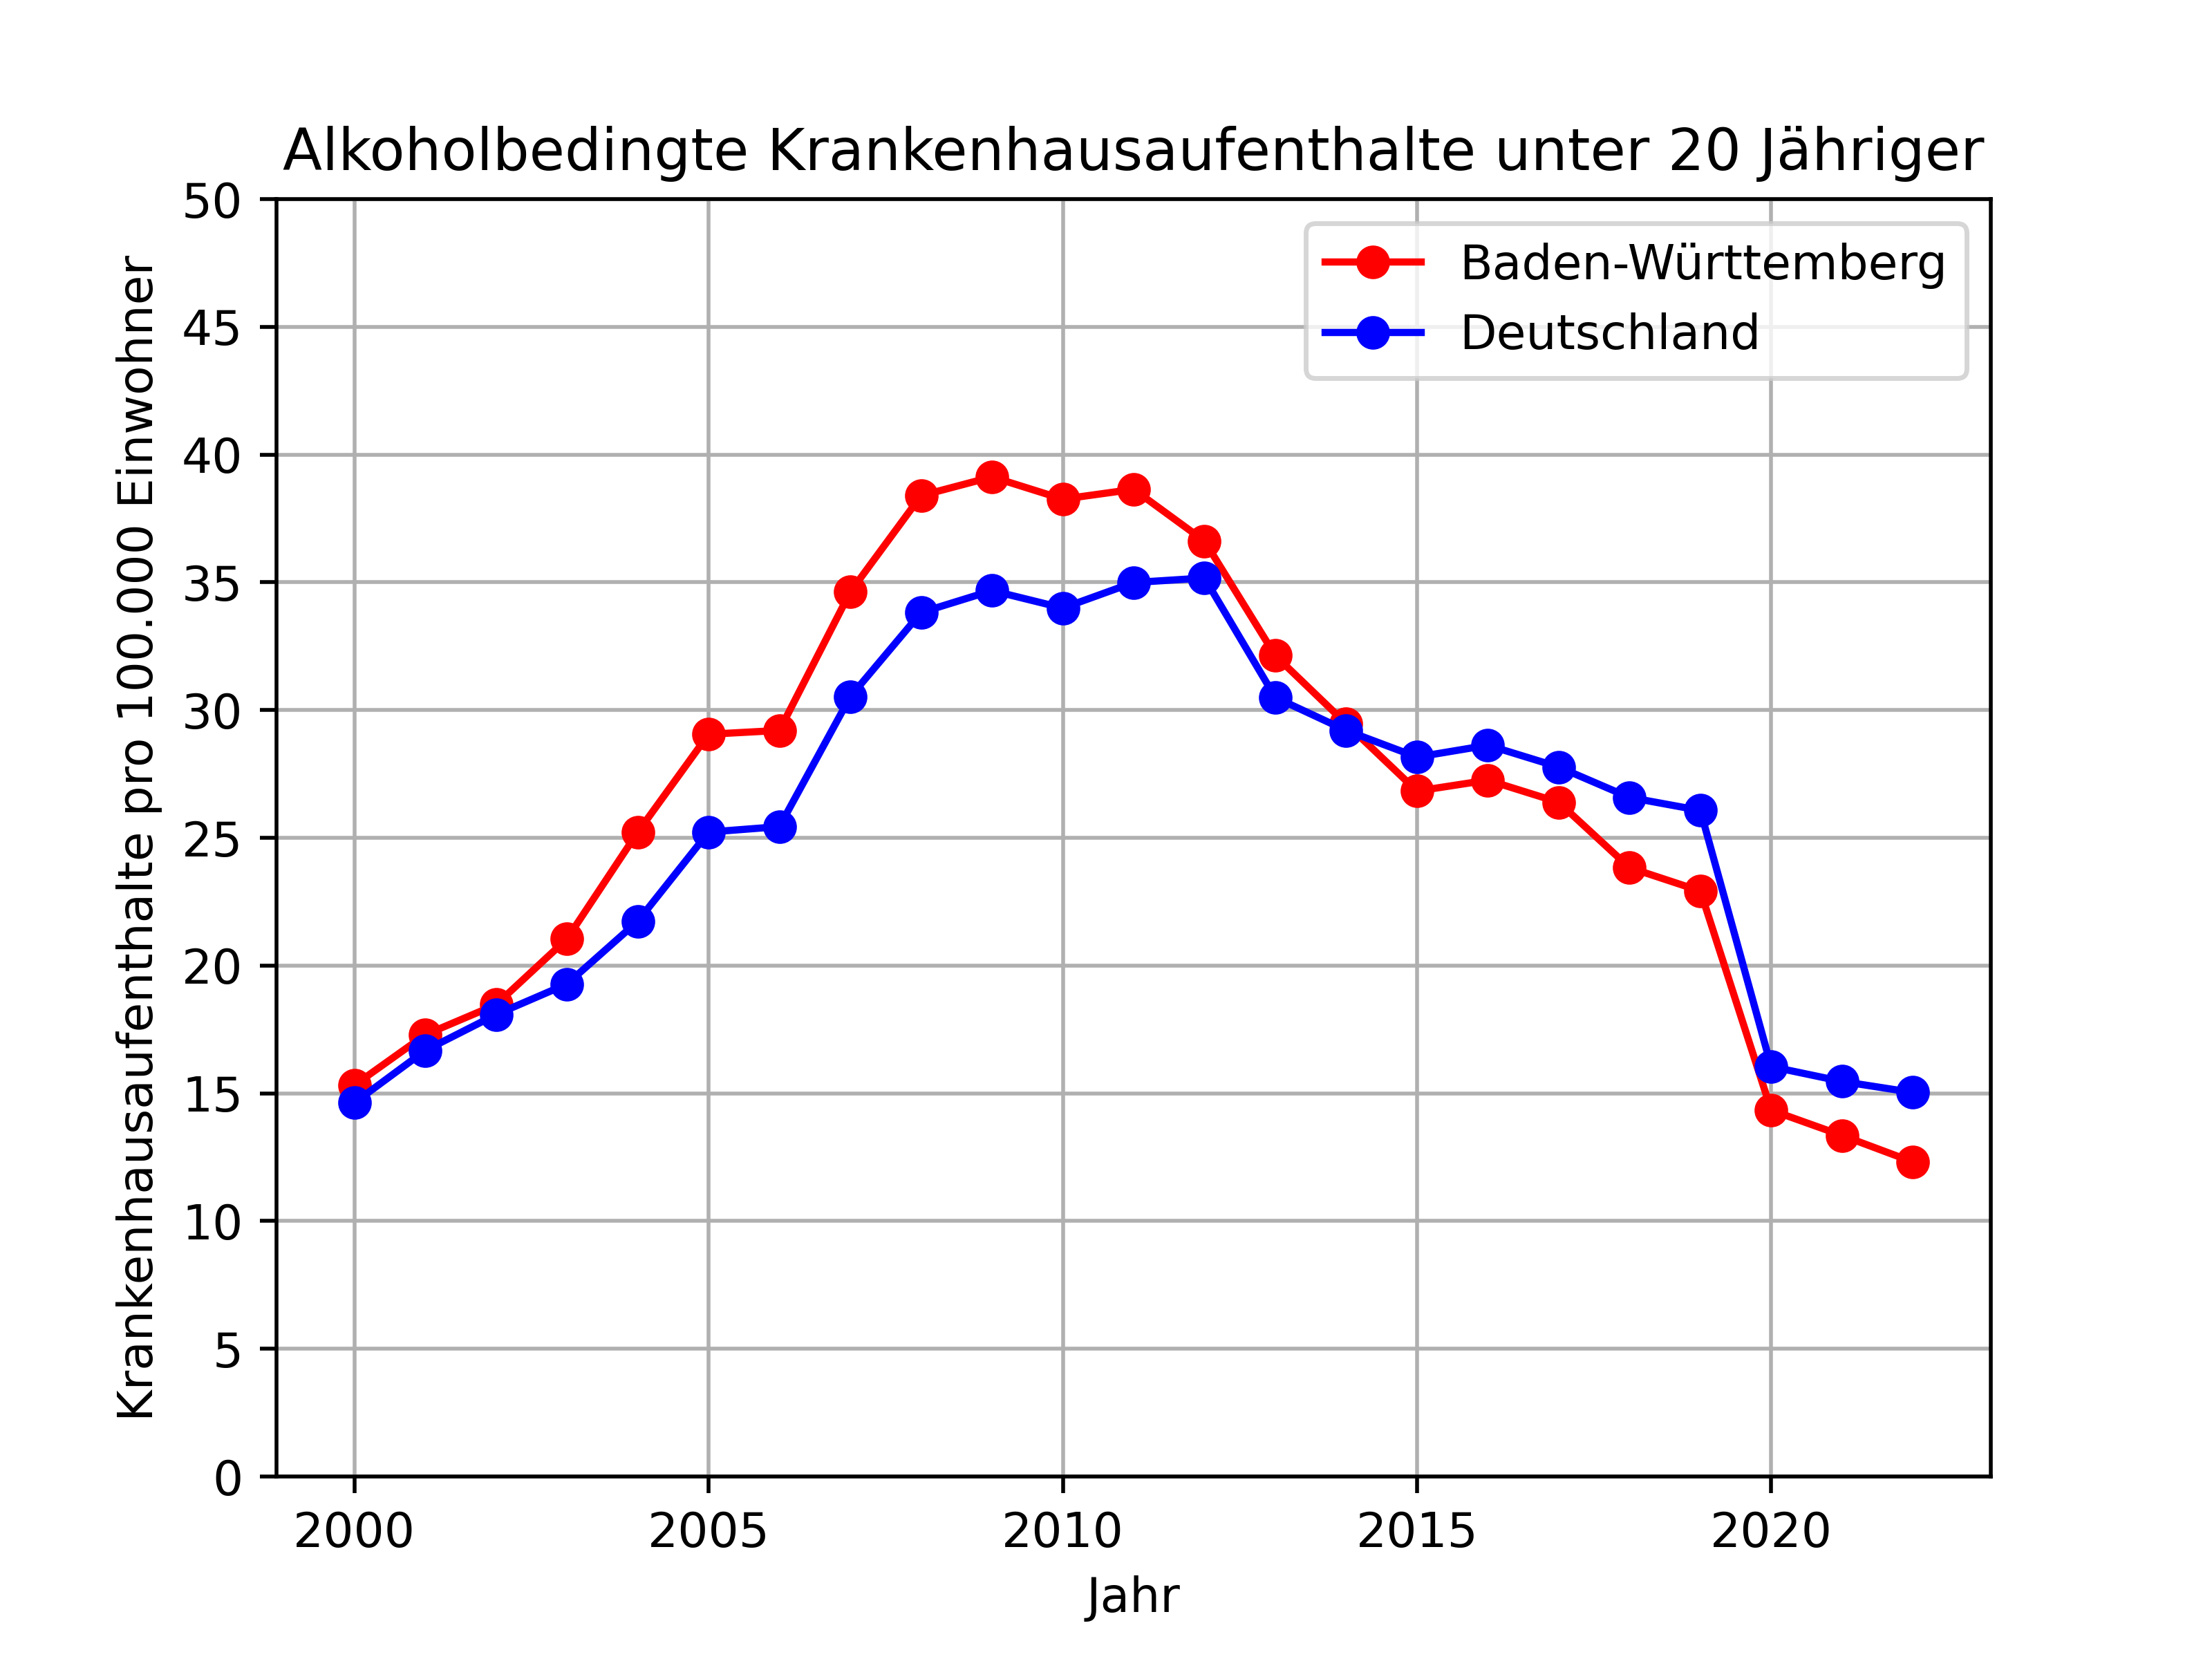
\includegraphics[scale=.7]{"assets/Alkohol_BW_Ges.png"}
    \caption{Alkoholbedingte Krankenhausaufenthalte von Jugendlichen von 2000 bis 2022}
    \label{fig:Krankenhausaufenthalte_3}
\end{figure}
Diese Grafik wurde ebenfalls mit den oben genannten Methoden erstellt.
Man sieht dass sich die Verläufe von Baden-Baden Württemberg und Deutschland stark ähneln. Sie erreichen bis 2010 Höchstwerte und fallen bis 2019 auf ein Niveau von ca. 25 Krankenhausaufenthalte pro 100.000 Einwohner ab. Auch der Einfluss der Corona-Pandemie auf diesen Verlauf ist sehr gut zu erkennen, die Werte aus den Jahren 2020, 2021 und 2022 sind deutlich geringer als die der Jahre davor. Sogar die Tagesschau berichtet von derartigen Effekten \autocite{tagesschaude_weniger_nodate}.

\section{Eigene Umfrage}
Eigene Umfrage 
In unserer Seminararbeit geht es auch viel um das Vergleichen des Alkoholkonsums in verschiedenen Personen- und Altersgruppen. Deshalb fanden wir es interessant uns ein Bild von unserem eigenen Umfeld zu machen. 
Befragt wurden alle Schüler der Klasse 10 sowie der Jahrgansstufen 1 und 2. Insgesamt haben 101 der 129 Schüler an der Umfrage teilgenommen, was einer Beteiligung von ungefähr 78 Prozent entspricht.  
31 Stimmen sind von der Jahrgangsstufe 2, somit machen rund 30 Prozent aller Beteiligten aus. Am meisten teilgenommen haben die Schüler der Jahrgangsstufe 1. Hier haben sich 40 Schüler (39,6\%) die Zeit genommen um die Fragen zu beantworten. Rein von der Anzahl der Teilnehmer nahmen am wenigsten Schüler der Klasse 10 teil. Von Ihnen haben 30 Schüler an der Umfrage teilgenommen. 
Jedoch muss man berücksichtigen, dass in der Klassenstufe 10 deutlich weniger Schüler sind, als in den anderen Stufen. Somit ist der prozentuale Anteil der teilnehmenden Schüler in Klasse 10 mit 77\% wiederum am zweithöchsten nach der Jahrgangsstufe 1 (83\% aller Schüler in dieser Stufe). Die Jahrgangsstufe 2 hatte sich mit 73\% dennoch ebenfalls sehr gut an der Umfrage beteiligt. 
Für uns sehr passend ist die ausgeglichene Beteiligung von männlichen und weiblichen Schülerinnen und Schüler, es ermöglicht uns die Resultate auf beide Geschlechter zu beziehen. 50 Schüler stehen in der Umfrage 49 Schülerinnen gegenüber, während lediglich 2 keine Angabe zu ihrem Geschlecht geben wollten. 
Vor dem Absenden der Umfrage haben wir uns vorgestellt, dass die meisten zwischen 14 und 15 das erste Mal Alkohol getrunken haben und diese Vermutung wurde letztendlich auch bestätigt. Über die Hälfte haben in diesem Zeitraum ihren ersten Kontakt zu Alkohol gehabt, wobei auch mit 13 relativ viele Schüler abgestimmt haben. Nur selten wurde bereits in jüngerem oder älterem Alter schon getrunken. Auch interessant, ganze 14 Leute haben noch nie Alkohol getrunken. 
Bei der Frage, wie oft die Abgefragten aktuell noch trinken ist das Ergebnis ziemlich ausgeglichen. Zwischen ,,seltener als einmal im Monat“ und ,,häufiger als einmal in der Woche“ gibt es abgesehen von ,,mehrmals im Monat“ (24\%) kaum prozentuale Unterschiede (zwischen 11\% - 15\%). Von den ursprünglich 14 Schülern, welche noch nie Alkohol getrunken haben, trinken zwischenzeitlich neun Weitere keinen Alkohol mehr. Das bringt uns zu dem Schluss, dass manche einmal probiert und danach aber nichts mehr getrunken haben, wobei aber sicherlich auch welche dabei sind, die einfach so aufgehört haben. Dafür kann es verschiedene Anlässe geben, beispielsweise aus körperlichen oder gesundheitlichen Gründen wie einer entstandenen Allergie. 
Etwas überraschend fanden wir, dass Mischgetränke und purer Schnaps mit Abstand am beliebtesten waren. Knapp 70 Prozent trinken sehr gerne Mischgetränke, wenn sie auf einer Party sind und mit 39 Prozent trinken die Befragten am zweitmeisten Schnaps (Shots), was doch ein deutlicher Abstand zu Bier, welches am dritt-­beliebtesten ist (32\%). Etwas irritierend fanden wir allerdings, dass bei dieser Frage nur noch 22 Leute mit "keinen Alkohol“ abgestimmt haben. Wir konnten es uns nur so erklären, dass diese eine Person abgestimmt hat, welches Getränk sie früher am liebsten getrunken hat. 



\section{Problem}
Im ersten Teil haben wir ausführlich erfahren, dass Alkohol vor allem bei Jugendlichen und jungen Erwachsenen sehr schädlich ist. 
 %(TODO ggf bezug auf zeit)
In der obigen Analyse von verschiedenen Statistiken haben wir herausgefunden, dass es zwar keine signifikanten Unterschiede zwischen der konsumierten Alkoholmenge in Nord- und Süddeutschland gibt. Insgesamt wird in Deutschland aber sehr viel Alkohol konsumiert, auch im weltweiten Vergleich. Laut der WHO wurden in Deutschland 2019 durchschnittlich 12.2 Liter Reinalkohol pro Kopf konsumiert, mehr als doppelt so viel wie der globale Durchschnitt von 5.5 Litern pro Kopf \autocite{noauthor_alcohol_nodate-1}. In Deutschland starben allein 2016 62.000 Menschen an allein auf Alkohol zurückzuführende Todesursachen \autocite{noauthor_alkoholkonsum_nodate}. Dafür bekommt Deutschland von der WHO einen YLL score von 3 von 5 \autocite{noauthor_alcohol-attributable_nodate }. Der YLL (years of life lost) score gibt die durchschnittliche Anzahl an Lebensjahren an, die durch einen vorzeitigen Tod durch eine Krankheit oder andere Todesursache im Vergleich zu der durchschnittlichen Lebenserwartung der Bevölkerung verloren wurde \autocite{martinez_reflection_2019}. Die WHO gibt mit ihrem score an, welcher Anteil des YLL scores der jeweiligen Bevölkerung durch Alkohol verursacht wurde. 1 ist hierbei der geringste Anteil, 5 der höchstmögliche.
Ein wichtiger Faktor für diesen hohen Alkoholkonsum ist vermutlich die unkritische Einstellung der Gesellschaft gegenüber Alkohol \autocite{noauthor_alkoholkonsum_nodate}. Das zeigt sich daran, dass weiten Kreisen der Gesellschaft alltäglicher Alkoholkonsum üblich ist, z.B. in Form von einem "Feierabendbier" oder einem "Verdauungsschnaps" oder einem "Gläschen Wein zur Tagesschau". Auch auf vielen Festen im süddeutschen Raum ist Alkoholkonsum ein wichtiger Aspekt. Das beste Beispiel hierfür ist natürlich das bayrische Oktoberfest, aber auch auf den meisten lokalen Festen wie z.B. Schützen oder dem Öchslefest ist der Alkohol für viele gar nicht wegzudenken. Diese unkritische Einstellung gegenüber von Alkohol fängt natürlich schon bei Jugendlichen an, auf denen auch der Fokus unserer Seminararbeit liegt. () TODO ggf bezug auf Iserv Statistik). Auch in der obigen Analyse der Krankenhausstatistik haben wir herausgefunden, dass in deutschland eine signifikante Anzahl an jugendlichen aufgrund von einer Alkoholintoxikation im Krankenhaus behandelt werden muss. Die Anzahl der Jugendlichen, die große Mengen an Alkohol trinken, deswegen aber nicht im krankenhaus behandelt werden müssen ist natürlich dementsprechend viel größer (TODO bezug auf Iserv statikstik). Daher beschäftigen wir uns im folgenden mit verschieden Methoden um Jugendliche vor der Gefahr des Alkohols zu beschützen. 

\subsection{Prävention}

TODO studie zu prävention zotero

\subsection{Verbote}
Weitreichende Verbote sind für den Alkoholkonsum von jugendlichen in Deutschland keine wirksame und sinnvolle Lösung. Nehmen wir an, das Mindestalter für den Alkoholkonsum wird um zwei Jahre erhöht, d.h. Bier, Wein und Sekt dürften erst ab 18 Jahren konsumiert werden. Ein solches Verbot bräuchte einen großen Rückhalt in der Gesellschaft, da Jugendliche unter 18 Jahren sonst durch Eltern oder ältere Bekannte einfach an Alkohol gelangen könnten. Auch den erhöhten Reiz, den ein Verbot auf Jugendliche haben kann, darf man nicht außer Acht lassen \autocite{skala_jugend_2020}. 
Allein an unserer Iserv-Umfrage und an der Krankenhausstatistik kann man deutlich erkennen, dass ein solches Verbot nur einen geringen Effekt haben würde. Von den Schülern der Stufe 10, 11 und 12 die bereits einmal Alkohol getrunken haben haben nur 10\% mit 16 oder älter das erste mal Alkohol getrunken. 
% TODO satz nicht so scheiße formulieren 





TODO quelle empfehlungen für eltern vom Gesundheitsministerium sehr gut

TODO werbung für alkohol
\printbibliography
\end{document}
